\documentclass[12pt,letterpaper,USenglish]{article}

\usepackage[most]{tcolorbox}
\usepackage{amsmath}
\usepackage{amssymb}
\usepackage{microtype}
\usepackage{tikz}
\usepackage{paralist}
\usetikzlibrary{calc,positioning,backgrounds,intersections,graphdrawing,shapes,graphs,arrows,arrows.meta,chains}
\usegdlibrary{trees}

%%% Please use define.org for macros.
\input{define.orgtex}

\def\tikznbb#1;{\tikz{\useasboundingbox (0, 0) rectangle (0, 0);#1;}}

\begin{document}

\tikzset{lead/.style={anchor=north west,font=\it\bfseries,text=algs4red},
  treenode/.style={draw, minimum
      height=13pt, fill=white,inner sep=3pt, font=\footnotesize,
      rounded rectangle},
    algs4arrow/.style={->,>={Latex[length=7pt]},line width=0.8mm,algs4red},
    graphs/mytree/.style= {
    tree layout,
    sibling distance=5mm, level distance=5mm,
    nodes={treenode},
    edges={thick}},
  gnode/.style={draw,circle,treenode,font=\ttfamily\footnotesize},
  algs4arrow/.style={->,>={Latex[length=7pt]},line width=0.8mm,algs4red},
  redlink/.style = {algs4red, line width=3pt},
  heading/.style = {text width=20cm, fill=algs4red,text=white, align=left,
  font=\sffamily\bfseries}}


\lstset{deletedelim=**[is][]{!}{!}}

\noindent\begin{tikzpicture}[every node/.style={anchor=north west},remember picture]
  % Main background
  \begin{scope}[on background layer]
    \fill[black!10!white, draw=white, line width=6pt] (-.5\textwidth, 0) rectangle (.5\textwidth, -18cm);
  \end{scope}

  % Clip and left margin
  \path [save path=\theframe, rounded corners] ($(-.5\textwidth, 0) + (1.5pt,-1.5pt)$)
  rectangle ($(.5\textwidth, -18cm) + (-1.5pt, 1.5pt)$);
  \clip [use path=\theframe];
  \coordinate (left) at ($(-.5\textwidth, 0) + (0.3cm,0)$);

  % Title
  \node [anchor=north,text width=20cm,minimum height=1.4cm,align=center,fill=algs4red,text=white]%
  {\sffamily\Large \textbf{4.1}\quad UNDIRECTED GRAPHS: TRAVERSALS};


  %% Glossary lead
  \node [heading] (glos) at (-.5\textwidth,-1.3cm) {~~Depth-first search (DFS)};
  \newcommand{\indentrule}{\color{gray!60}\rlap{\smash{\hspace{9pt}\rule[-.35em]{.7pt}{1.45em}}}}

  \def\mph#1{\emph{\color{algs4red}#1}}
  \node at ($(glos.south west) + (0.3cm, -0cm)$) {\begin{minsizebox}{20.2cm}{10cm}
      \begin{lstalgs4}#i
public class DepthFirstSearch
  private Set<Integer> marked =
  			 new Set<> ();
  public DepthFirstSearch (Graph G, int s)
    dfs (G, s);
  
  private void dfs (Graph G, int v)
    marked.add (v);
    for (int w : G.adj (v))
      if (!marked.contains (w)) dfs (G, w);
  
  public boolean isMarked (int w) 
    return marked.contains (w);
\end{lstalgs4}
\end{minsizebox}
};
  \node at ($(glos.south west) + (9.4cm, -.2cm)$)
  {\begin{minsizebox}{9.3cm}{10cm}
      \noindent \mph{\textbf{Applications.}}\\
      \begin{compactitem}
    \item \mph{Connectivity}: marked after DFS means connected.
    \item \mph{Finding paths}: can store ``parent'' while recursing.
      \item \mph{Connected components}: restart DFS on unmarked nodes.
      \item \mph{Cycle}: if DFS sees a marked node that is not the parent.
      \item \mph{\(2\)-colorable}: alternate colors in DFS.
      \end{compactitem}
    \end{minsizebox}};
  \node at ($(glos.south west) + (11.6cm, -4.6cm)$) {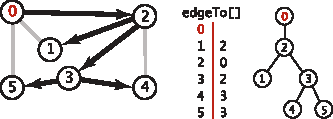
\includegraphics[height=2cm]{dfs}};

  %% Glossary lead
  \node [heading] (glos) at (-.5\textwidth,-9.1cm) {~~Breadth-first search (BFS)};
  \node at ($(glos.south west) + (0.3cm, -0cm)$) {\begin{minsizebox}{20.2cm}{10cm}
      \begin{lstalgs4}#i
public class BreadthFirstSearch
  private Set<Integer> marked =
  			 new Set<> ();
  public BreadthFirstSearch (Graph G, int s)
    Queue<Integer> queue = new Queue<> ();
    queue.enqueue (s);
    while (!queue.isEmpty ())
      int v = queue.dequeue ();
      if (!marked.contains (v))
        marked.add (v);
        for (int w : G.adj (v))
          queue.enqueue (w);
  
  public boolean isMarked (int w)
    return marked.contains (w);
      \end{lstalgs4}
    \end{minsizebox}};
  \node at ($(glos.south west) + (9.4cm, -.2cm)$)
  {\begin{minsizebox}{9.3cm}{10cm}
      \noindent \mph{\textbf{Applications.}}\\
      \begin{compactitem}
      \item \mph{All of the above}.
      \item \mph{Shortest path}: as direct neighbors are seen first, this
        computes shortest path.
      \end{compactitem}
      \vspace{1cm}
      \noindent \mph{\textbf{Note.}} Swapping \lstinline{Stack} for
      \lstinline{Queue} turns BFS into DFS.
    \end{minsizebox}};
  \node at ($(glos.south west) + (10.9cm, -4.6cm)$) {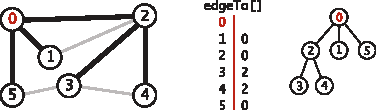
\includegraphics[height=2cm]{bfs}};
  %% Box
  \draw [algs4red,line width=3pt] [use path=\theframe];

\end{tikzpicture}
\end{document}
